\documentclass[a4paper]{article}
\usepackage[margin=3cm]{geometry}
\usepackage[utf8]{inputenc}
\usepackage{cmbright}
\usepackage[hidelinks]{hyperref}
\usepackage{booktabs}
\usepackage[ngerman]{babel}
\usepackage{parskip}
\usepackage{graphicx}
\usepackage{minted}
\usepackage{pdflscape}
\usepackage{array}
\usepackage{tabulary}
\usepackage{multicol}
\usepackage{pgfgantt}
\usepackage{pgf-umlcd}
\usepackage{enumitem}

% Page breaks between sections
\let\oldsection\section
\renewcommand\section{\clearpage\oldsection}

% JIRA/Confluence shortcuts
\def\jiraurl{https://jira.keltec.ch/jira}
\def\confluenceurl{https://jira.keltec.ch/wiki}
\newcommand{\jiraissue}[1]{\href{\jiraurl/projects/EPJ/issues/EPJ-#1}{EPJ-#1}}
\newcommand{\fulljiraissue}[1]{EPJ-#1 (\url{\jiraurl/projects/EPJ/issues/EPJ-#1})}

% Tools
\newcommand{\tool}[2]{\emph{#1\footnote{\url{#2}}}}

\begin{document}
	\title{
		Projekt: kitovu \\
		\Large{Software-Architektur} \\[3em]
		
\includegraphics[width=20em]{../../img/logo/kitovu.jpg}
	}
	\author{
		Florian Bruhin \\ \url{florian.bruhin@hsr.ch} \and
		Méline Sieber \\ \url{meline.sieber@hsr.ch} \and
		Nicolas Ganz \\ \url{nicolas.ganz@hsr.ch} 
		}
	\date{\today}
	
	\maketitle

\section*{Änderungsgeschichte}

\begin{tabulary}{\linewidth}{llLl}
	\toprule
	Datum & Version & Änderung & AutorIn \\
	\midrule
	28.03.2018 & 1.0 & Dokument erstellt, Grundgerüst von Template übernommen & Méline Sieber \\
	04.04.2018 & 2.0 & Abgabe End of Elaboration & alle \\

	\bottomrule
\end{tabulary}
\pagebreak

\section{Einführung}
Dieses Dokument schliesst die Entwicklungsphase ``End of Elaboration'' ab. Es legt dar, wie die Software-Architektur von \emph{kitovu} aufgebaut ist, beschreibt die logischen Schichten und deren Zusammenhänge. Zudem klärt es die grössten Risiken des Projekts, namentlich die Einbindung der beiden externen, als optional beschriebene Plattformen (Studentenportal, Moodle). Das Dokument erläutert auch die Herausforderung, die grafische Benutzeroberfläche mit dem Kommandozeilen-Client zu verbinden (Prozesse und Threads). Als letzter Punkt wird der Aspekt der Datenspeicherung, insbesondere der Aufbau der Konfigurationsdatei besprochen.

Es bleibt eine Anmerkung: Viele Punkte der ``End of Elaboration'' definiert schon der sehr ausführliche Projektplan. Um dieses Dokument möglichst schlank zu halten, werden deshalb gewisse Punkte aussen vor gelassen, insbesondere die Ausführungen zur Grösse und Leistung von \emph{kitovu}. Für diesen Punkt sei auf den Projektplan verwiesen.

\subsection{Gültigkeitsbereich}
Die vorliegende Architekturbeschreibung ist für das Engineering-Projekt im Frühlingssemester 2018 gültig. Falls dem Projekt grössere Veränderungen widerfahren, wird das Dokument dementsprechend angepasst. Umfassende Änderungen werden am Anfang des Dokuments protokolliert.

\subsection{Referenzen}
Die Anforderungsspezifikation ist eng mit der Domainanalyse und anderen Dokumenten verbunden. Die folgende Tabelle listet die wichtigsten Referenzen auf.

\begin{tabulary}{\linewidth}{Ll}
	Confluence & \url{\confluenceurl} \\
	Draw.io & \url{https://www.draw.io/} \\
	Github-Repository von \emph{kitovu} & \url{https://github.com/kitovu-bot/kitovu} \\
	JIRA	& \url{\jiraurl} \\
	Moodle & \url{https://moodle.hsr.ch} \\
	Moodle Desktop & \url{https://download.moodle.org/desktop/} \\
	OpenHSR Connect & \url{https://github.com/openhsr/connect} \\
	Studentenportal & \url{https://studentenportal.ch/} \\
	Switch AAI \newline (Authentication and Authorization Infrastructure)& \url{https://www.switch.ch/aai/} \\
\end{tabulary}

Beim Logo auf der Titelseite handelt es sich um eine stark überarbeitete Version eines GIFs (\url{https://www.animateit.net/details.php?image_id=8990}). Urheber und Copyright sind nicht auffindbar.

\pagebreak

\section{Systemübersicht}

Das folgende Kontextprogramm verdeutlicht, wie die Schnittstellen von \emph{kitovu} aussehen. Auf der einen Seite  sind die Nutzerinnen und Nutzer, die je nach Informatikkenntnissen mit der grafischen Oberfläche oder mit dem Kommandozeilenprogramm interagieren. Auf der andere Seite sind die Plattformen, die \emph{kitovu} einbindet: Der Skripteserver sowie die Moodle-Plattform, die jedoch eine Authentifikation via Switch AAI verlangt. Weshalb das Studentenportal für dieses Projekt nicht implementiert werden kann, erklärt der nächste Abschnitt.

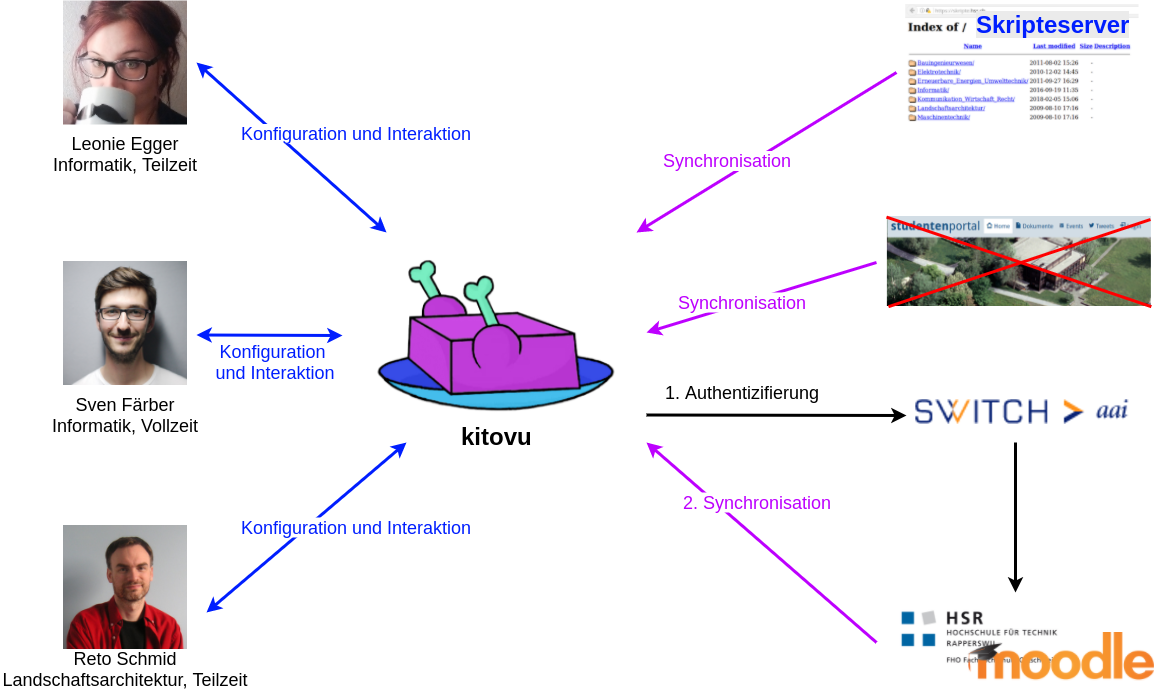
\includegraphics[width=40em]{./img/kontextdiagramm.png}

% <Beschreibt die Softwarearchitektur eines Systems und wie sie sich präsentiert (am besten mit einem Bild um eine Übersicht zu ermöglichen) und einzelne Beschreibungen zu den einzelnen Elementen des Systems>



\section{Architektonische Ziele und Einschränkungen}

Der Projektplan erläuterte bereits die beiden grössten Risiken: Die Einbindung des Studentenportals und von Moodle, so dass sich von beiden Plattformen auch Dokumente synchronisieren lassen.

Zum Ende der Elaborationsphase zeigt sich, dass diese frühzeitige Einschränkung des Projekts sinnvoll war: Die Abklärung mit dem OpenHSR-Verein und den Betreibern des Studentenportals ergab, dass wir darauf verzichten müssen, das Portal einzubinden. Es fehlt an einer API, mit der wir Files synchronisieren könnten -- wir müssten dies von Hand hinzufügen, was jenseits des Projektumfangs liegt. Zudem sind viele Komponente des Studentenportals veraltet und sollten dringend aktualisiert werden. Ein möglicher Sprint sollte dem Abhilfe schaffen. Doch diesen organisiert die Fachschaft oder der OpenHSR-Verein und ist somit ausserhalb unseres Projekts. Das Studentenportal wird somit kein Teil von \emph{kitovu}.

Das zweite Risiko, die Moodle-Einbindung, ist noch in weiterer Abklärung. Ein erster Erfolg konnte verzeichnet werden: Der Moodle-Desktop-Client\footnote{\url{https://download.moodle.org/desktop/}} bzw. die mobile Version davon stellt bei erfolgreichem Login einen Moodle-Token zur Verfügung. Dank dieses Tokens ist es uns gelungen, via \emph{kitovu} ein File herunterzuladen. Eine erste Anbindung ist uns also gelungen. Noch offen ist, wie und ob wir die direkte Authentifikation via Switch AAI in \emph{kitovu} implementieren können; wir sind jedoch zuversichtlich, dass uns das gelingt.

\subsection{Wichtige Abläufe}

Synchronisationsprozesse haben einen kritischen Punkt: Die Datenintegrität. Denn die Dateien sollen immer den Zustand behalten oder annehmen, wie die Nutzerin es wünscht. Um das zu gewährleisten, haben wir die Funktionalität des \verb|FileCache| definiert -- er führt Buch über den Zustand der Dateien\footnote{Vgl. auch Kapitel 6.}. Nach längeren Diskussionen haben wir folgende mögliche Fälle identifiziert, die während des Synchronisationsprozesses auftreten können:

\begin{tabulary}{\linewidth}{lLLLLl}
	\toprule
		\bfseries Fall &
	    \bfseries Situation Remote &
	    \bfseries Situation Lokal &
	    \bfseries Situation &
	    \bfseries Vorgehen &
	    \bfseries Enum-Wert\\
	\midrule
1 & nichts vorhanden &	lokal A &	remote gelöscht &	Konfliktbehandlung (delete local file) & 	REMOTE*\\ \hline
2 & nichts vorhanden &	lokal A' &	remote gelöscht, lokal geändert&	Konfliktbehandlung &	BOTH*\\ \hline
3 & remote A &	nichts &	neue Datei existiert &	download &	REMOTE\\ \hline
4 & remote A &	lokal A &	keine Änderungen &	nichts& 	NONE\\\hline
5 & remote B (neue Folien) &	lokal A (keine Änderungen) &	Folien-Update vom Dozent &	download &	REMOTE\\\hline
6 & remote A &	lokal A' (lokal geändert) &	lokale Notizen, kein Folien-Update &	nichts &	LOCAL\\\hline
7 & remote B (neue Folien) &	lokal A' (lokal geändert) &	beides geändert &	Konfliktbehandlung &	BOTH\\\hline
8 & remote B &	lokal B &	FileCache nicht aktuell &	nichts tun, update FileCache &	NONE*\\\hline

\end{tabulary}

Die mit Sternchen (*) bezeichneten Einträge sind Spezialfälle. 

Aus der Tabelle wird ersichtlich, dass der \verb|FileCache| primär dazu da ist, festzustellen, ob es jemals lokale Änderungen gab (aus A wurde A'). Mit anderen Worten: Wir müssen A separat -- im \verb|FileCache| -- abspeichern, um später feststellen zu können, ob sich in der Zeit bis zum nächsten Synchronisationsprozess die Datei geändert hat. Daraus entstehen drei Digests:

\begin{itemize}
	\item Remote, der direkt aus der Remote-Datei berechnet wird
	\item Lokal im FileCache
	\item Lokal auf der Festplatte, i.e. der Digest, der direkt aus der Datei berechnet wird.
\end{itemize}

Der \verb|FileCache| wird jeweils geschrieben, wenn die Datei heruntergeladen wird, und enthält zwei Werte: Den Digest zum Zeitpunkt der Synchronisation sowie den lokalen Dateipfad samt Dateinamen.

Die oben definierten Enum-Werte REMOTE, LOCAL, BOTH, NONE verwenden wir, um die Konfliktbehandlung zu implementieren. Diese ist nötig, sobald sich die Datei lokal geändert hat (A').

In der derzeitigen Entwicklungsphase des Clients haben wir uns vorerst für die Konfkliktbehandlung ``override'' entschieden. Wenn sich also die Datei zwischen zwei Synchronisationsprozessen geändert hat, wird sie erneut von der Remote-Datei überschrieben.

Es ist uns jedoch ein Anliegen, dass sich diese Konfliktbehandlung von der Nutzerin steuern lässt, also dass sie in der Konfigurations von \emph{kitovu} festlegen kann, wie sich bei einem Konflikt das Programm verhalten soll (override, ignore, rename, ask).

\section{Logische Architektur}

% <Beschreibung der logischen Struktur des Projekts. Pro Subsystem/Package ein einzelner Abschnitt und ein Übersichtsdiagramm über die einzelnen Subsysteme/Packages. Aufteilung in Subsysteme/Packages (zum Beispiel: 3-Layer-Architektur mit GUI, Problem Domain und Datenhaltung). >

% Weitere Punkte: Klassenstruktur, Schnittstellen, Wichtige interne Abläufe, Wichtige Abläufe

\subsection{Schichten}

%FIXME: Nicolas korrigiert Fehler in Darstellung (moodledingens), fügt filecache und konfig-file ein

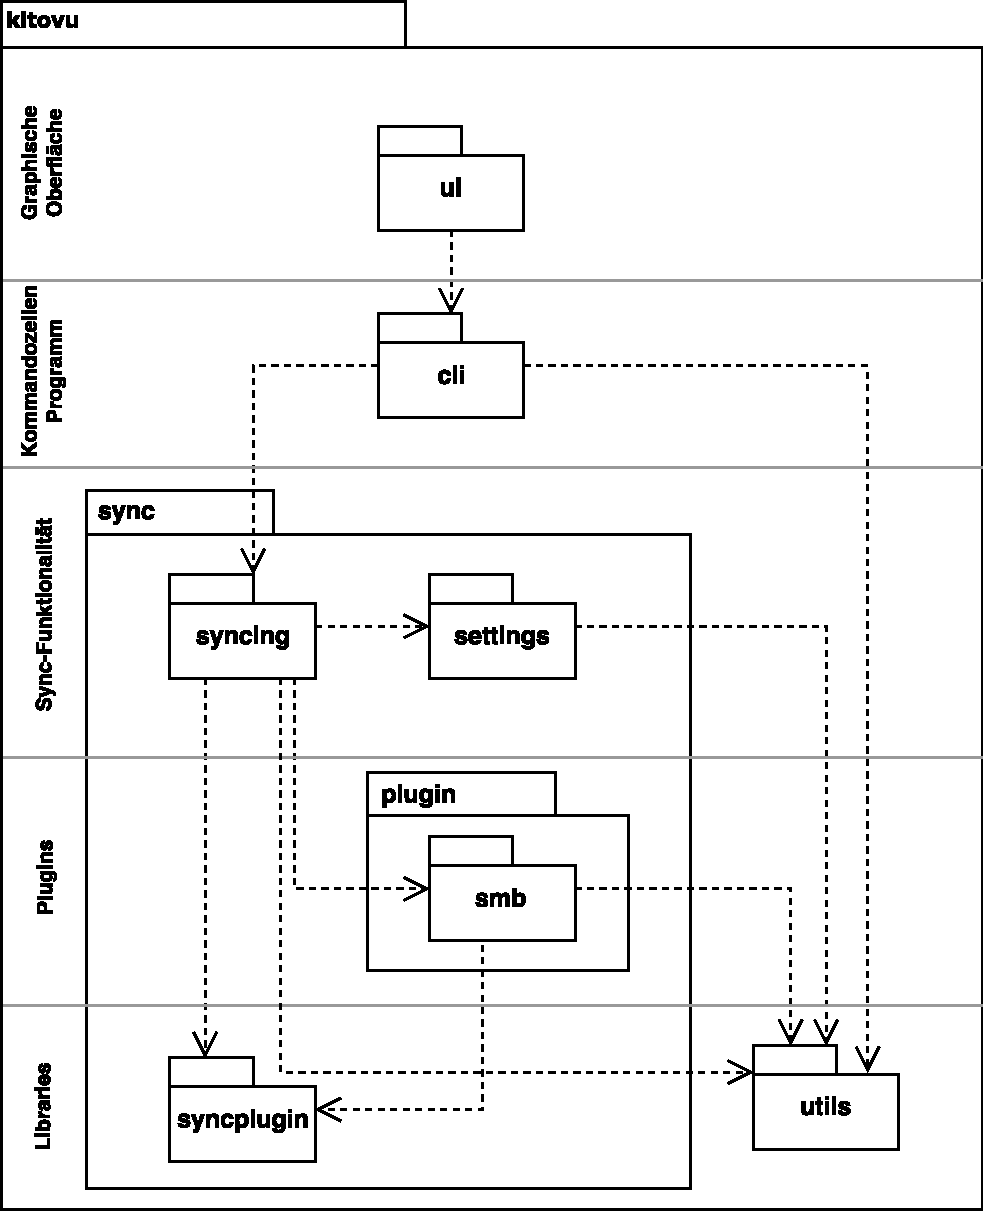
\includegraphics[width=40em]{./img/schichtendiagramm.pdf}

\subsection{Sequenzdiagramm}

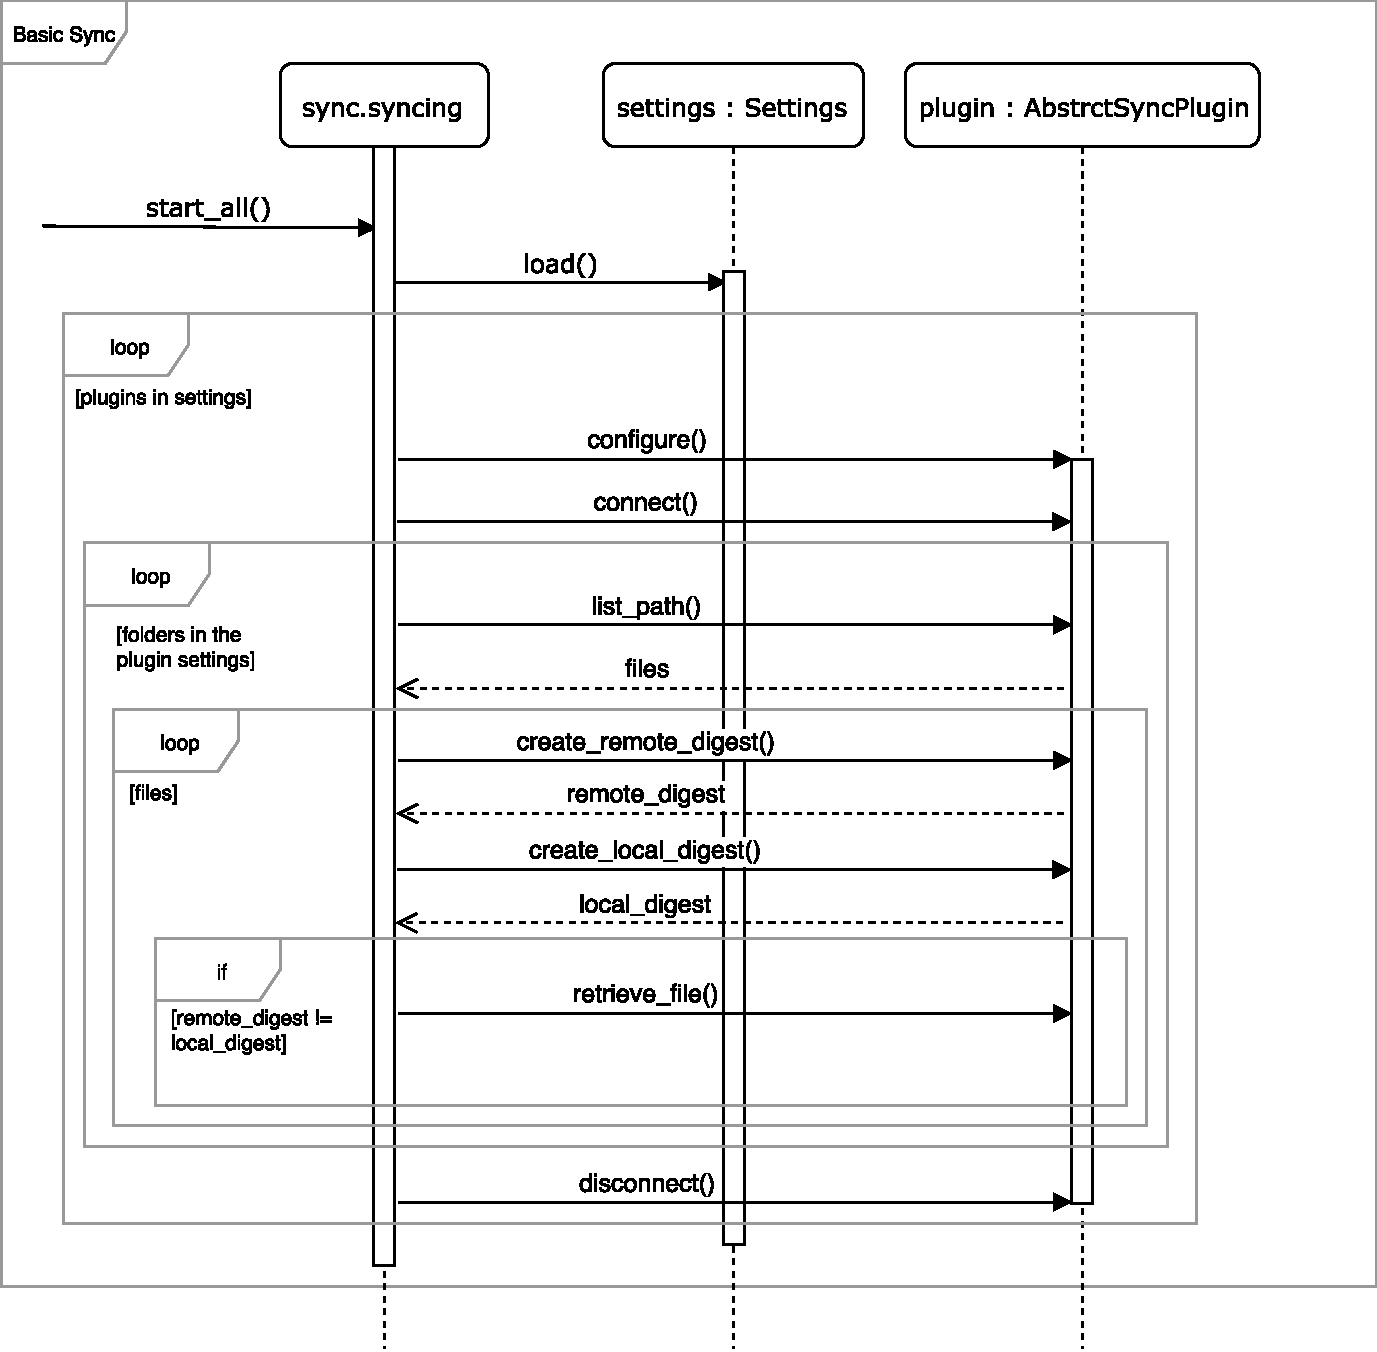
\includegraphics[width=40em]{./img/GrobesSequenzDiagramm.pdf}

\section{Prozesse und Threads}

% <Wenn mehrere Prozesse oder Threads eingesetzt werden wird hier beschrieben, wie diese ablaufen, miteinander funktionieren, Daten austauschen, sich synchronisieren, usw.>

Die grafische Implementation von \emph{kitovu} stellt uns vor die Herausforderung, wie die Bibliotheken zur Synchronisation in die GUI (die nicht blockiert werden darf) eingebunden werden. Dazu gibt es mehrere Lösungsansätze:

\begin{enumerate}
	\item Zwei separate Prozesse: Das GUI läuft in einem separaten Prozess und kommuniziert mit dem CLI-Prozess, der die Synchronisation übernimmt.
	\item Zwei Threads: Die Bibliotheken zur Synchronisation laufen in einem separaten Thread im gleichen Prozess wie die GUI.
	\item Verwenden von asynchronen Bibliotheken (\verb|asyncio| oder \verb|twisted|), die im gleichen Thread wie die GUI die Synchronisation durchführen können, ohne die GUI zu blockieren.
\end{enumerate}

Für den Kommandozeilen-Client nehmen wir in Kauf, dass der Client blockiert wird, wenn er die Synchronisation durchführt.

Für den GUI-Protoyp wählen wir die erste Lösung oben in der Liste. Der grafische und textbasierte Client implementieren wir also als zwei separate OS-Prozesse. Für ein besseres GUI sollte dies jedoch via Threads oder einer Python-Bibliothek für asynchrone Programmierung erfolgen (dritte Variante oben). Hier folgen wir dem Projektplan und nehmen an, dass diese Implementation nicht mehr Teil des Engineering-Projekts sein wird.

\section{Datenspeicherung}

% <Beschreibung mit Diagramm der Datenspeicherung (Datenmodell, z.B. Datenbank)>
\subsection{Konfigurationsdatei}
Die Konfigurationsdatei soll so gestaltet sein, dass auch Studierende ausserhalb des Informatikstudienganges damit umgehen könnten. Die Verständlichkeit steht also im Vordergrund. 

Wir folgen deshalb dem Vorschlag von Nicolas Ganz und wählen einen Plugin-Aufbau der Konfigurationsdatei.

\begin{minted}{yaml}

root-dir: ~/Documents/HSR/semester_06

global-ignore:
  - Thumbs.db
  - .DS_Store

plugins:
  - name: skripte-server
    type: samba
    # hostname: svm-c213.hsr.ch
    # port: 445
    # share: skripte
    username: nganz
    # ...

sync:
  - name: Engineering-Projekt
    plugins:
      - plugin: skripte-server
        ignored:
          - SubDir
          - example.txt
        remote-dir: Informatik/Fachbereich/Engineering-Projekt/EPJ
        # local-dir: Engineering-Projekt
\end{minted}

\subsection{FileCache}

Zum Bereich der Datenspeicherung gehört ebenfalls der \verb|FileCache|. Er ist im Wesentlichen eine lokale Speicherung des \verb|remote_digest|, der zum Zeitpunkt des letzten Synchronisationsvorgangs erstellt wurde. Anhand des \verb|FileCache| kann so zu einem späteren Zeitpunkt verglichen werden, ob sich bis dahin die lokale Datei geändert hat.

Da der \verb|FileCache| von einem erfolgreichen Synchronisationsprozess abhängig ist, existiert dazu noch kein Code im Prototyp beim derzeitigen Stand des Projekts. Im Gegensatz zur Konfigurationsdatei, die als \verb|YAML|-Datei gespeichert wird, speichern wir den \verb|FileCache| als \verb|JSON|-Datei. Der Vorteil einer \verb|JSON|-Datei ist die reduzierte Dateigrösse sowie bessere Performance. Zudem ist diese Datei nicht dazu gedacht, von Personen gelesen zu werden, in Kontrast zur Konfigurationsdatei.

Die Datei könnte folgendermassen aussehen:

\begin{minted}{json}
[{"plugin": "smb", "path": "EPJ/example.pdf", "digest": "123-12345"}]
\end{minted}

Gemäss unseren Berechnungen zu den Dateimengen in der Anforderungsspezifikation erwarten wir, dass diese Datei am Ende des Semesters rund 7000 Einträge umfasst, mit 1000 Einträgen pro Modul. Wir schätzen dies als eine handhabbare Grösse für den \verb|FileCache| ein.

\section{Skalierbarkeit}

\subsection{Mehr externe Plattformen}

Für das Engineering Projekt haben wir \emph{kitovu} in minimal möglichem Umfang geplant: Die Synchronisation mit dem Skripteserver muss funktionieren. Alle weiteren externen Plattformen haben wir als optional definiert, auch aufgrund möglicher Risiken -- die sich im Fall des Studentenportals als berechtigt erwiesen haben.

Wir wollten zudem von Beginn weg \emph{kitovu} so entwerfen, dass er sich leicht ausbauen lässt, da ja an der HSR die Unterrichtsmaterialien von verschiedenen Quellen synchronisiert werden. Eine weitere Überlegung war, dass künftige Studierende selber \emph{kitovu} erweitern können, so dass sie neue oder andere Plattformen selbständig einbinden können. Dies veranschaulicht bereits die Persona der Leonie Egger. 

Wir haben uns deswegen für eine Plugin-Architektur entschieden, so dass neue Plattformen einfach als neue Plugins geschrieben werden können, die dann in \emph{kitovu} eingehängt werden. So ist es theoretisch möglich, eine Vielzahl von externen Plattformen in \emph{kitovu} zu integrieren, ohne dass der gesamte Code umgeschrieben werden muss. Nachdem sich die ursprüngliche Plugin-Architektur \verb|pluggy| für Python als unbrauchbar erwiesen hatte, entschieden wir uns für \verb|stevedore|.\footnote{\url{https://docs.openstack.org/stevedore/latest/}}

Die geplante Erweiterbarkeit zahlt sich nun aus: Entgegen unseren kalkulierten Risiken ist eine Moodle-Anbindung möglich -- und lässt sich nun dank der Plugin-Architektur problemlos integrieren. \emph{Kitovu} skaliert also problemlos für mehr als eine Plattform.

\subsection{Mehr Nutzerinnen und Nutzer}

Vor und während der Projektarbeit haben wir festgestellt, dass \emph{kitovu} auf grossen Anklang stösst: Viele HSR-Studentinnen und -Studenten wünschen sich eine einfache Möglichkeit, ihre Unterrichtsmaterialien à jour zu halten. Wir hoffen deshalb und erwarten, dass der Client häufig und von vielen genutzt wird.

\emph{Kitovu} wird lokal bei den Nutzerinnen und Nutzern installiert, das Programm dürfte also problemlos skalieren, da mehr Nutzer keine grössere Last für den einzelnen Client bedeuten. Das einzige Problem wäre, dass die vielen Server-Anfragen von \emph{kitovu} den Skripteserver zum Erliegen bringen. Wir schätzen dieses Risiko jedoch als gering ein und erwarten von der Schulinfrastruktur, dass sie allfällige Spitzen von Netzwerkanfragen verarbeiten mag.

\end{document}
